\selectlanguage{english}
\begin{appendix}
\chapter{Appendix}

\section{Lua Codes}
\lstinputlisting[language=lua,breaklines=true,caption={Non Threaded child script to check distance},label={lst:check_distance}]{appendice/codes/check_distance.lua}

\section{Datasheets}

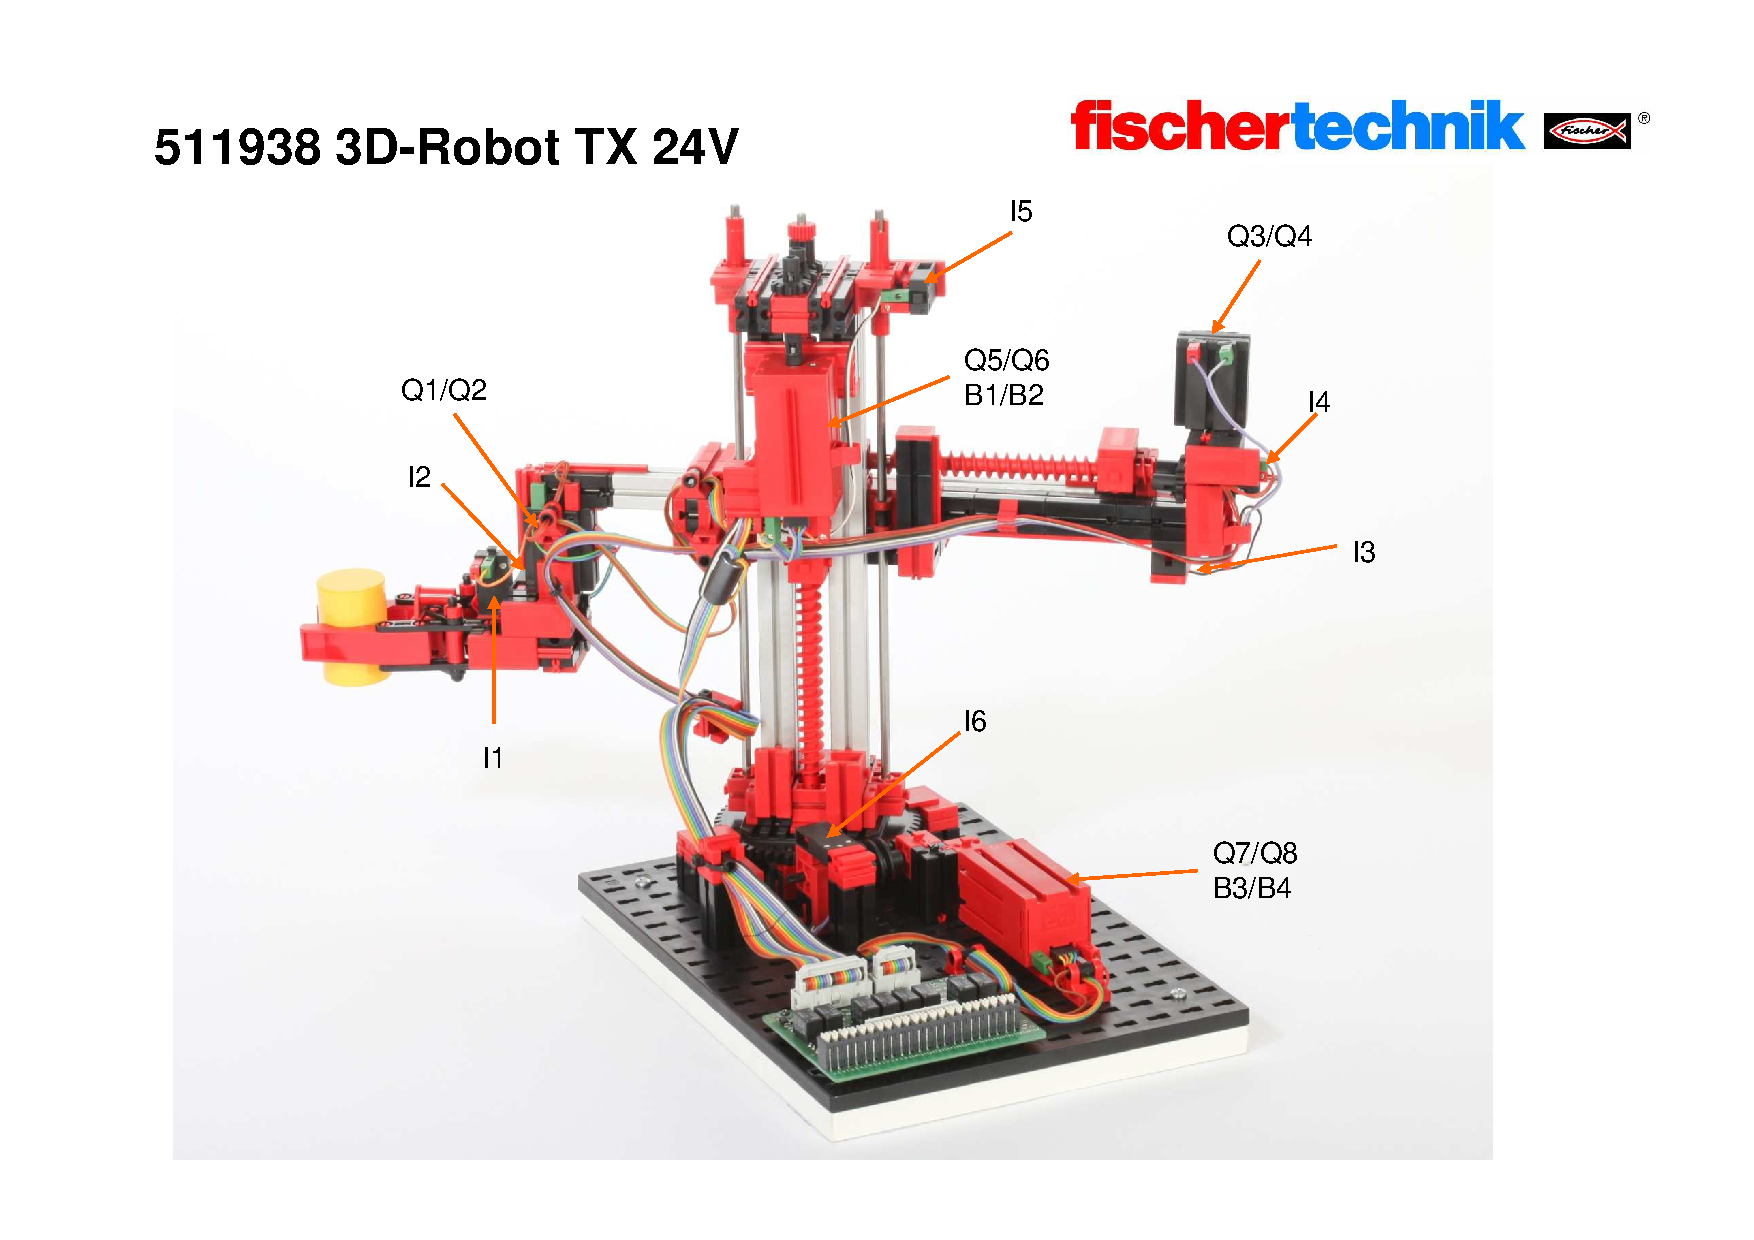
\includegraphics[width = 1\linewidth]{appendice/files/Robot.pdf}

\includepdf[pages={2,3,4}, scale =1]{appendice/files/Robot.pdf}

\includepdf[pages={2}, scale =1]{appendice/files/encoder.pdf}

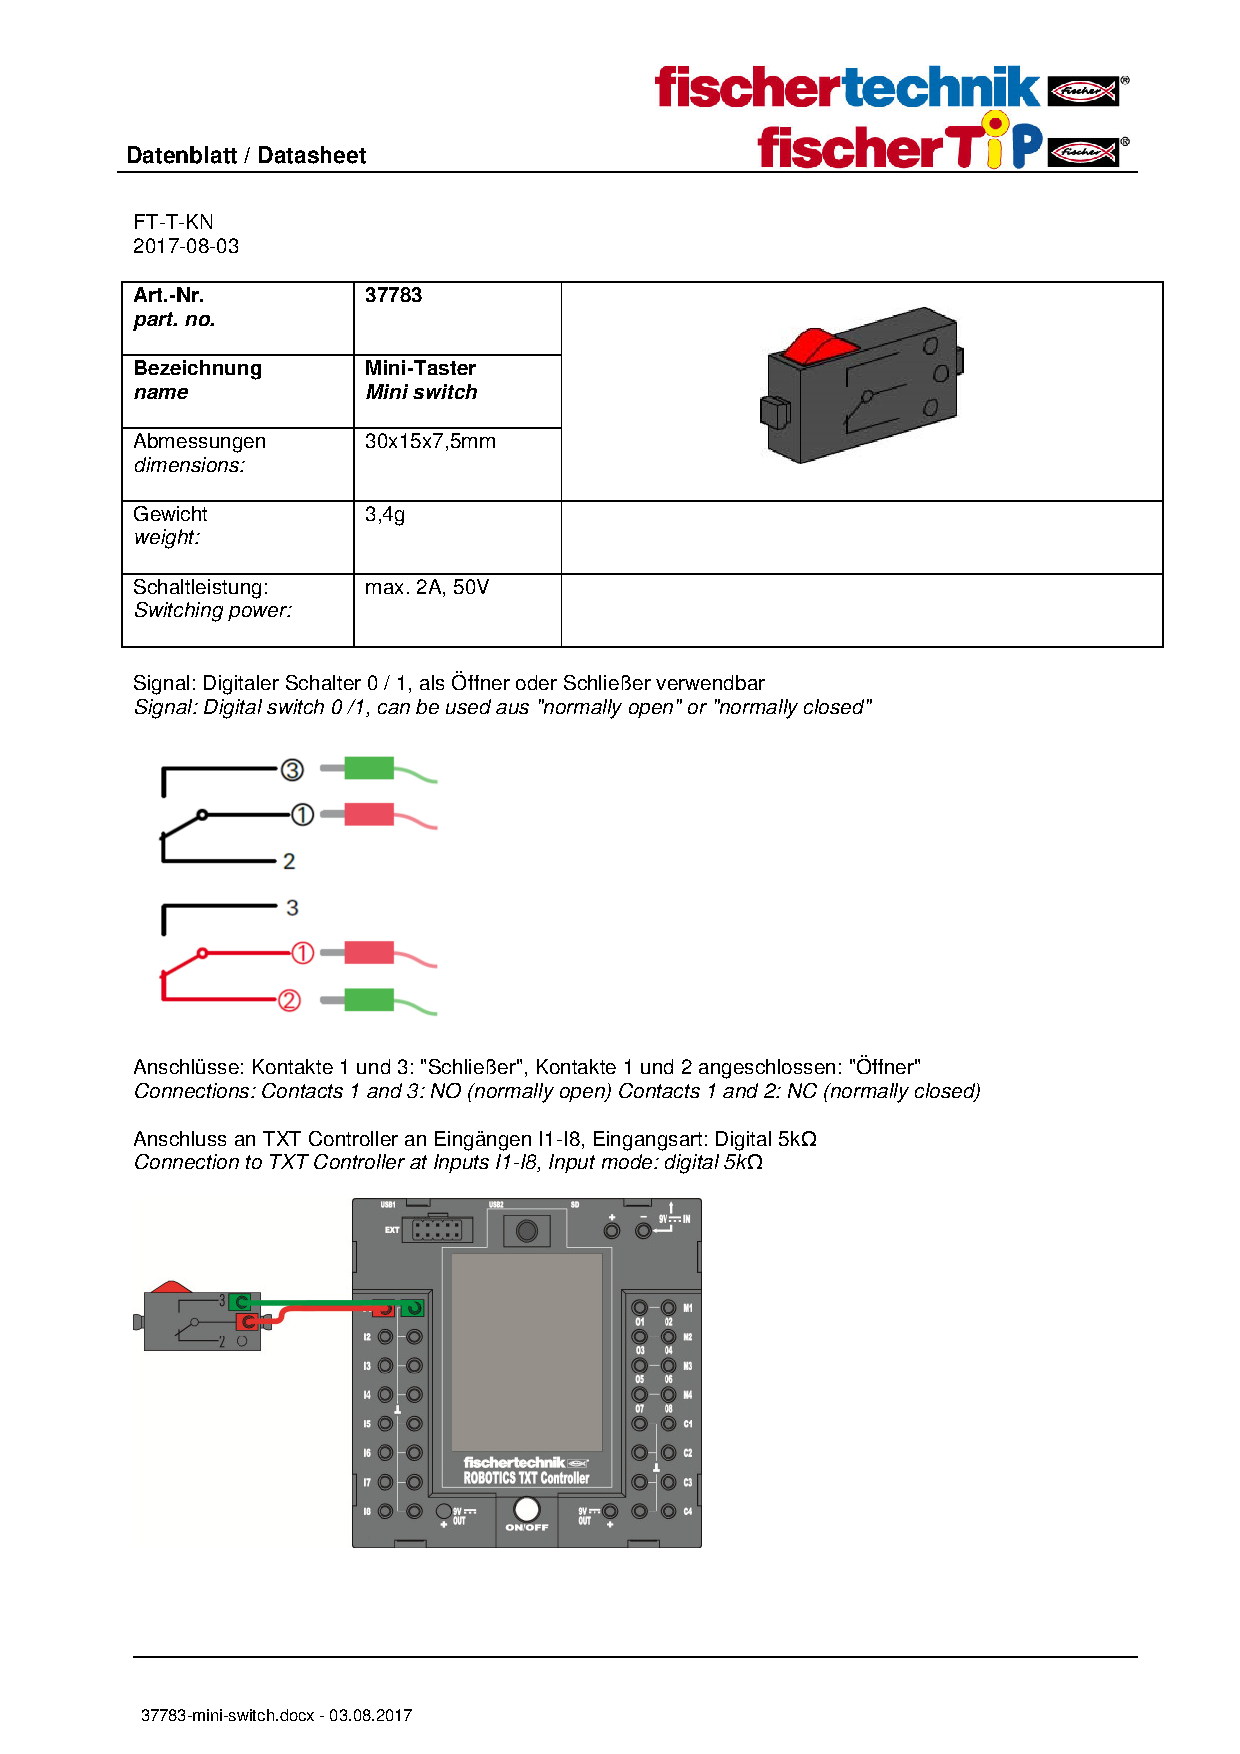
\includepdf[pages={-}, scale =1]{appendice/files/mini_switch.pdf}

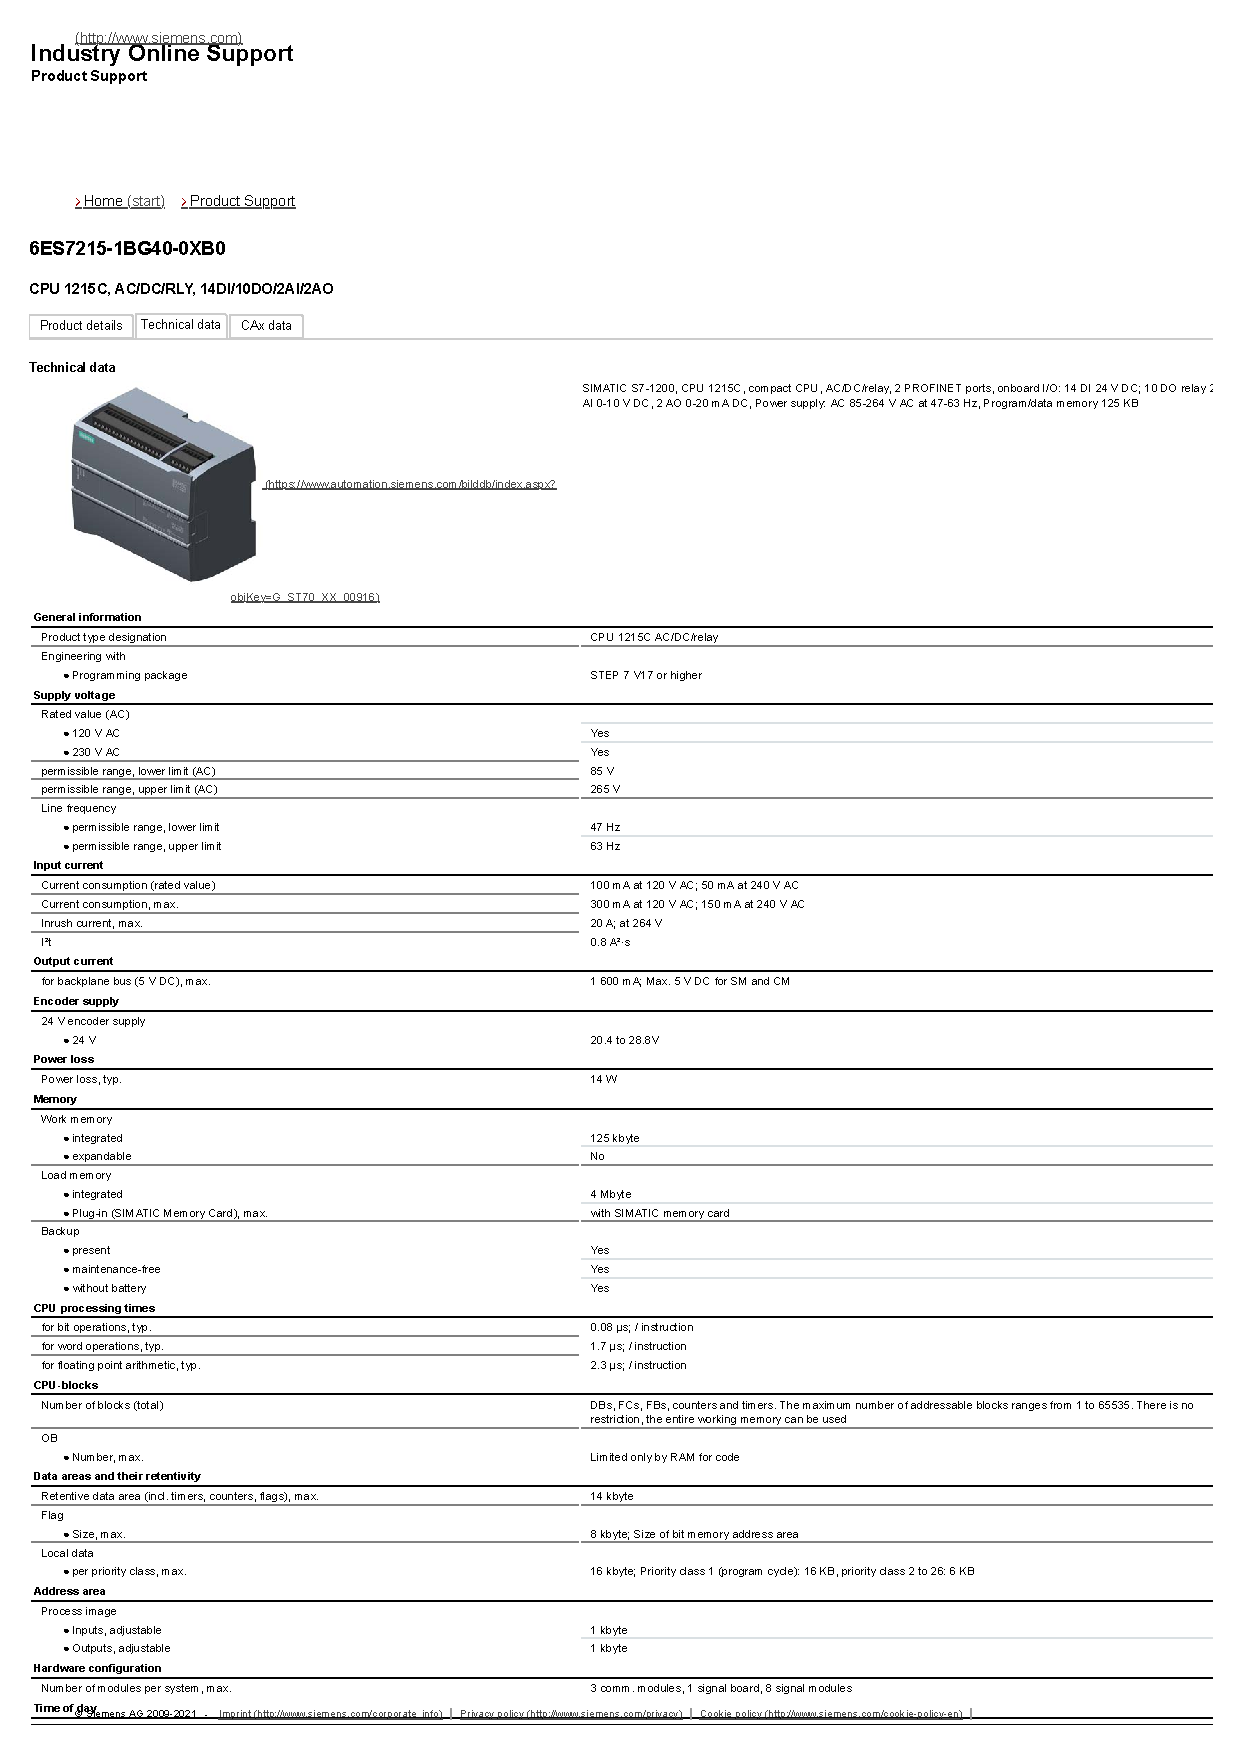
\includepdf[pages={1,2,3,4}, scale =1]{appendice/files/plc.pdf}

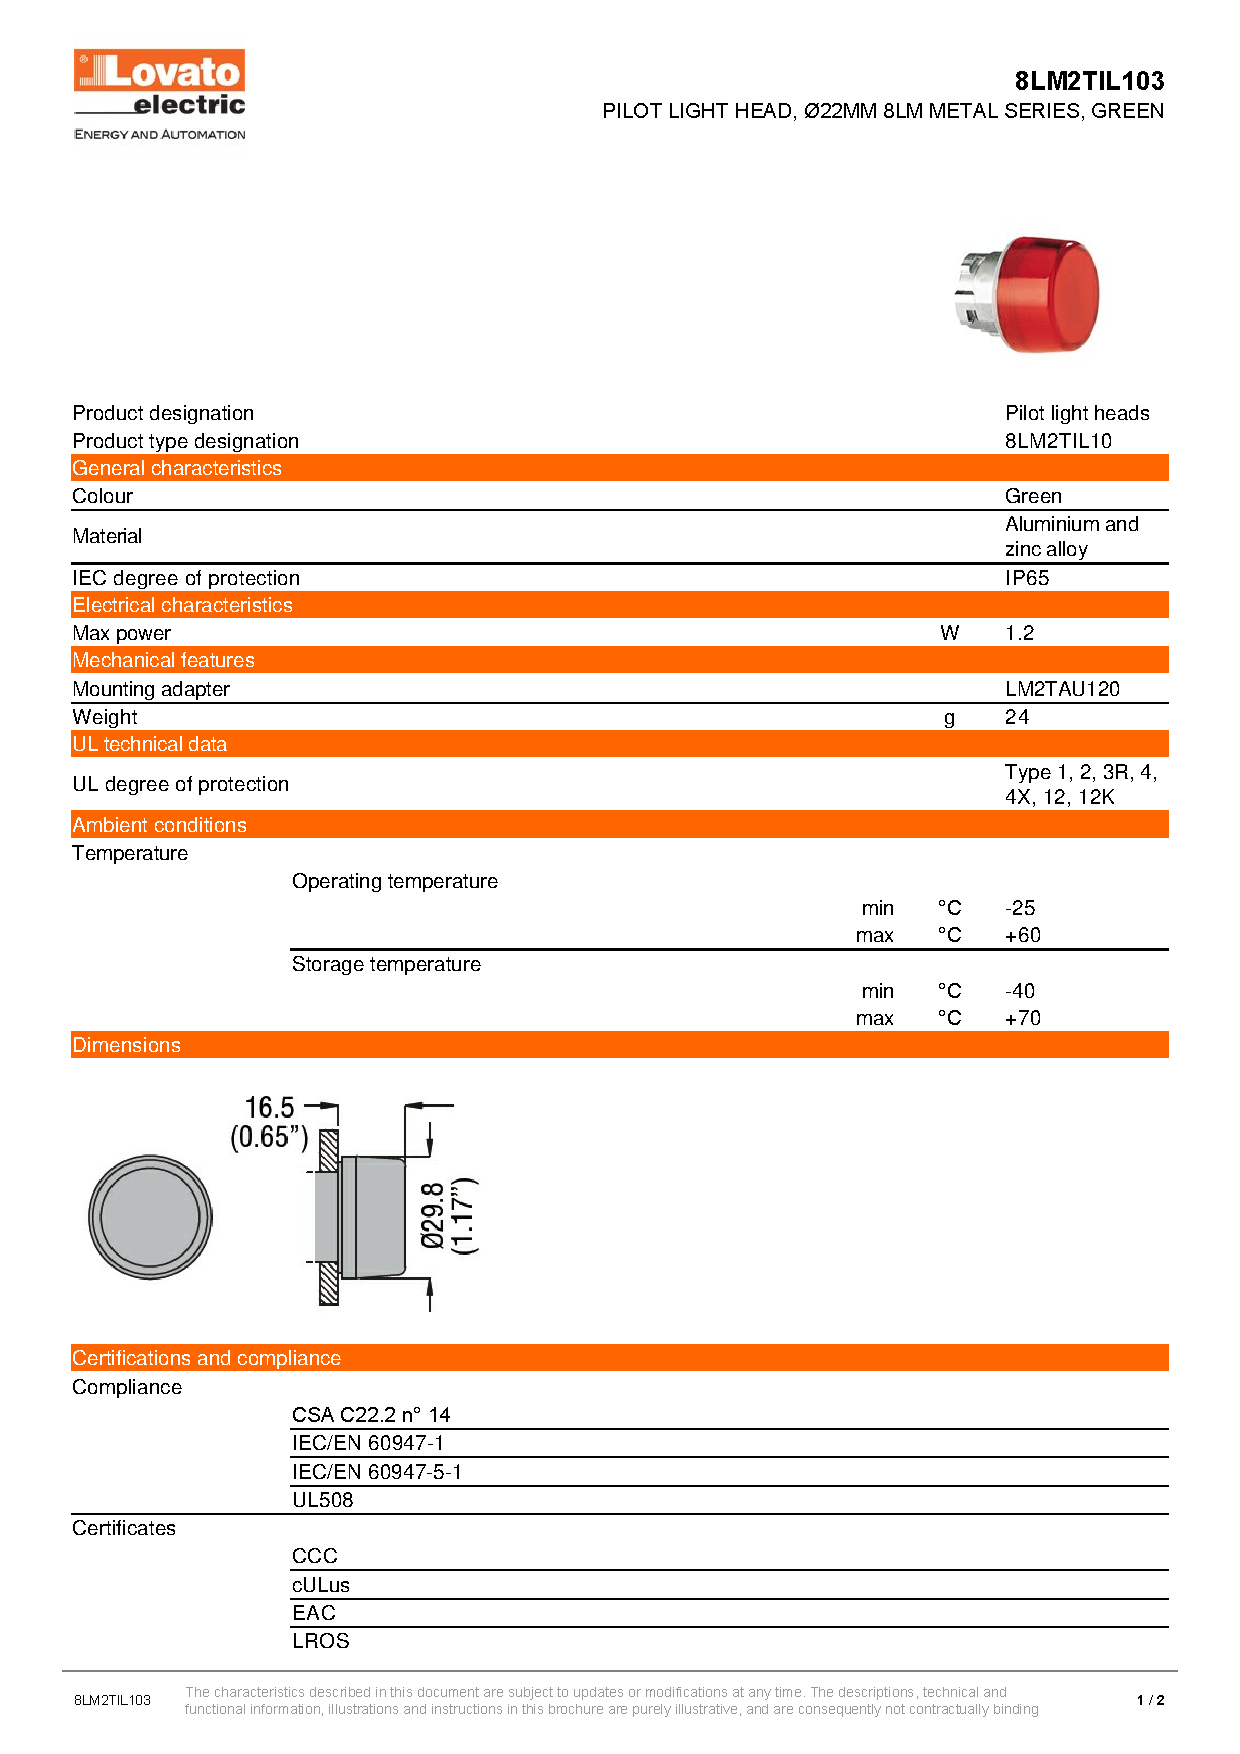
\includepdf[pages={-}, scale =1]{appendice/files/pilot_light_led_green.pdf}

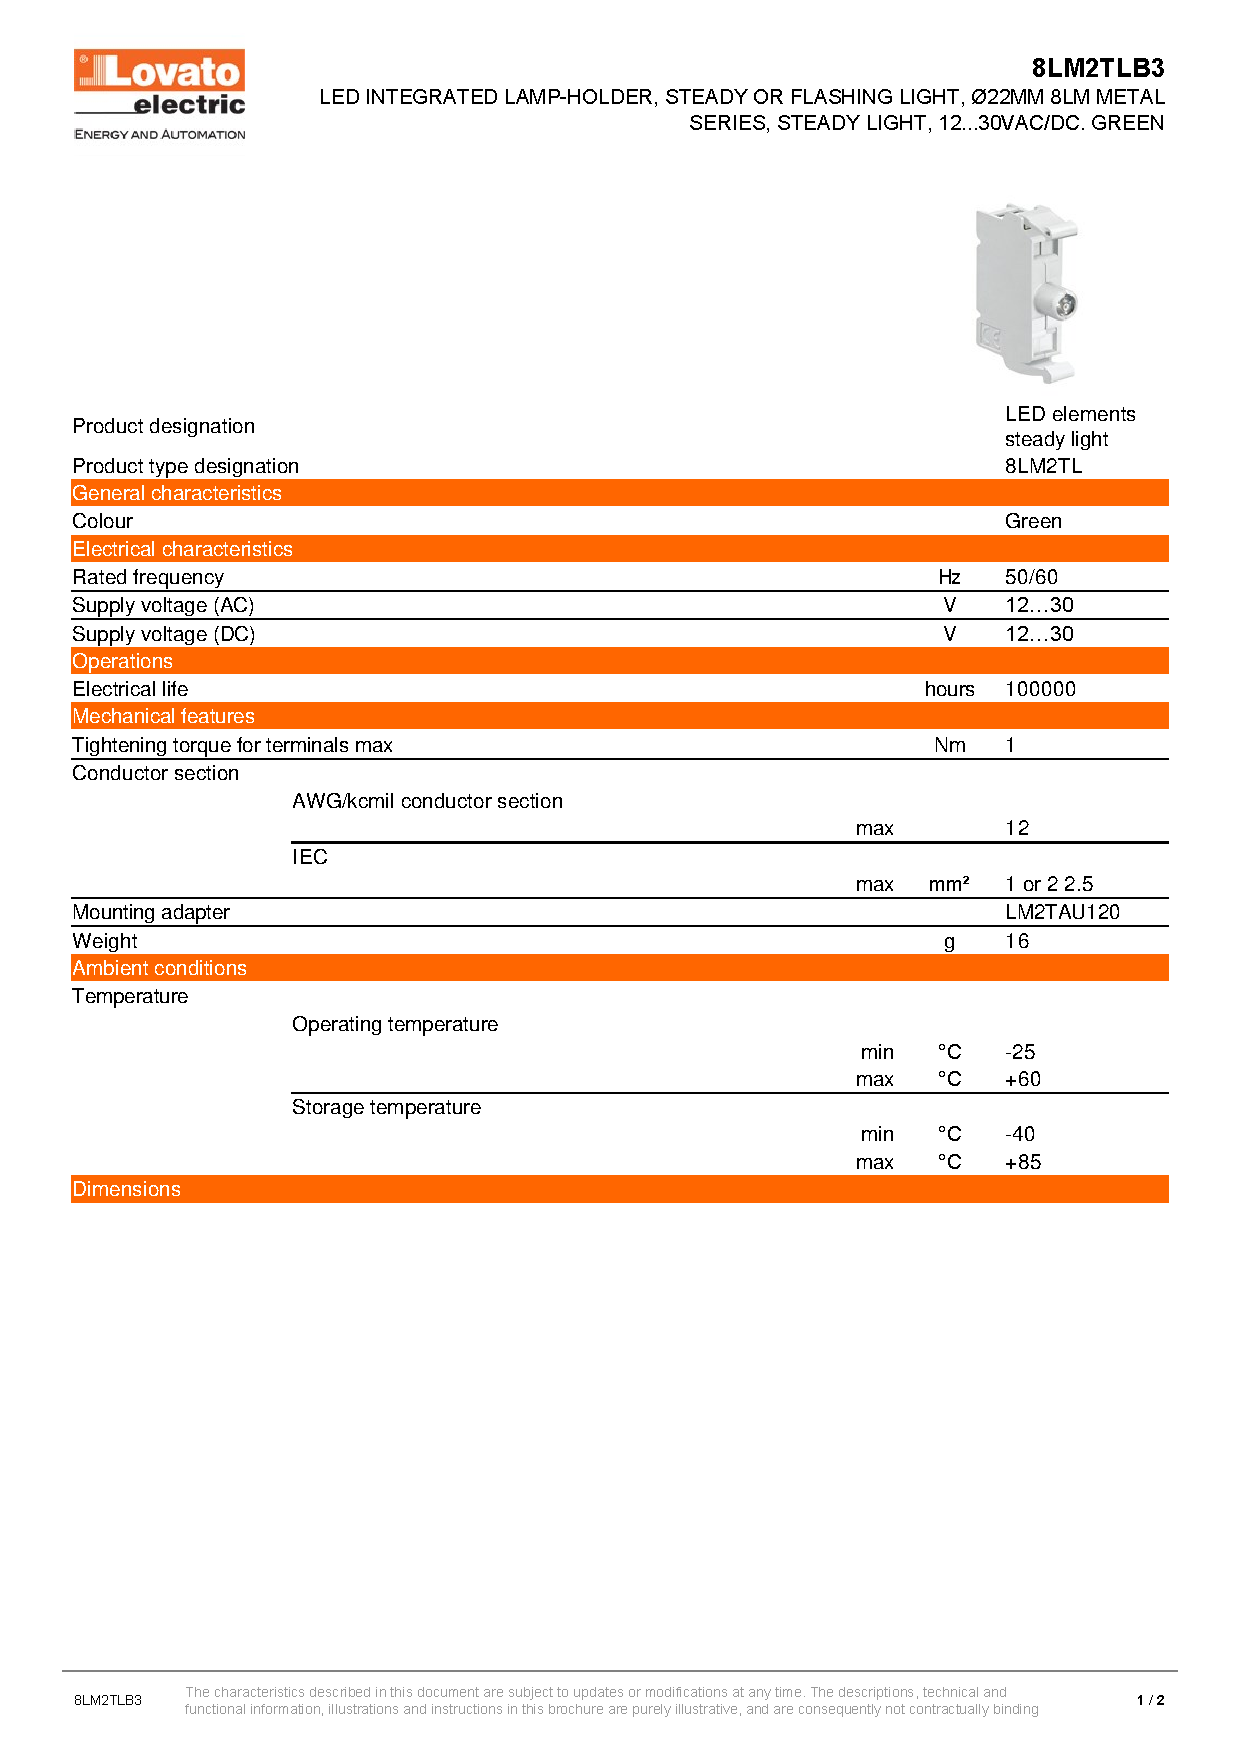
\includepdf[pages={-}, scale =1]{appendice/files/led_integrated_lamp_holder_green.pdf}

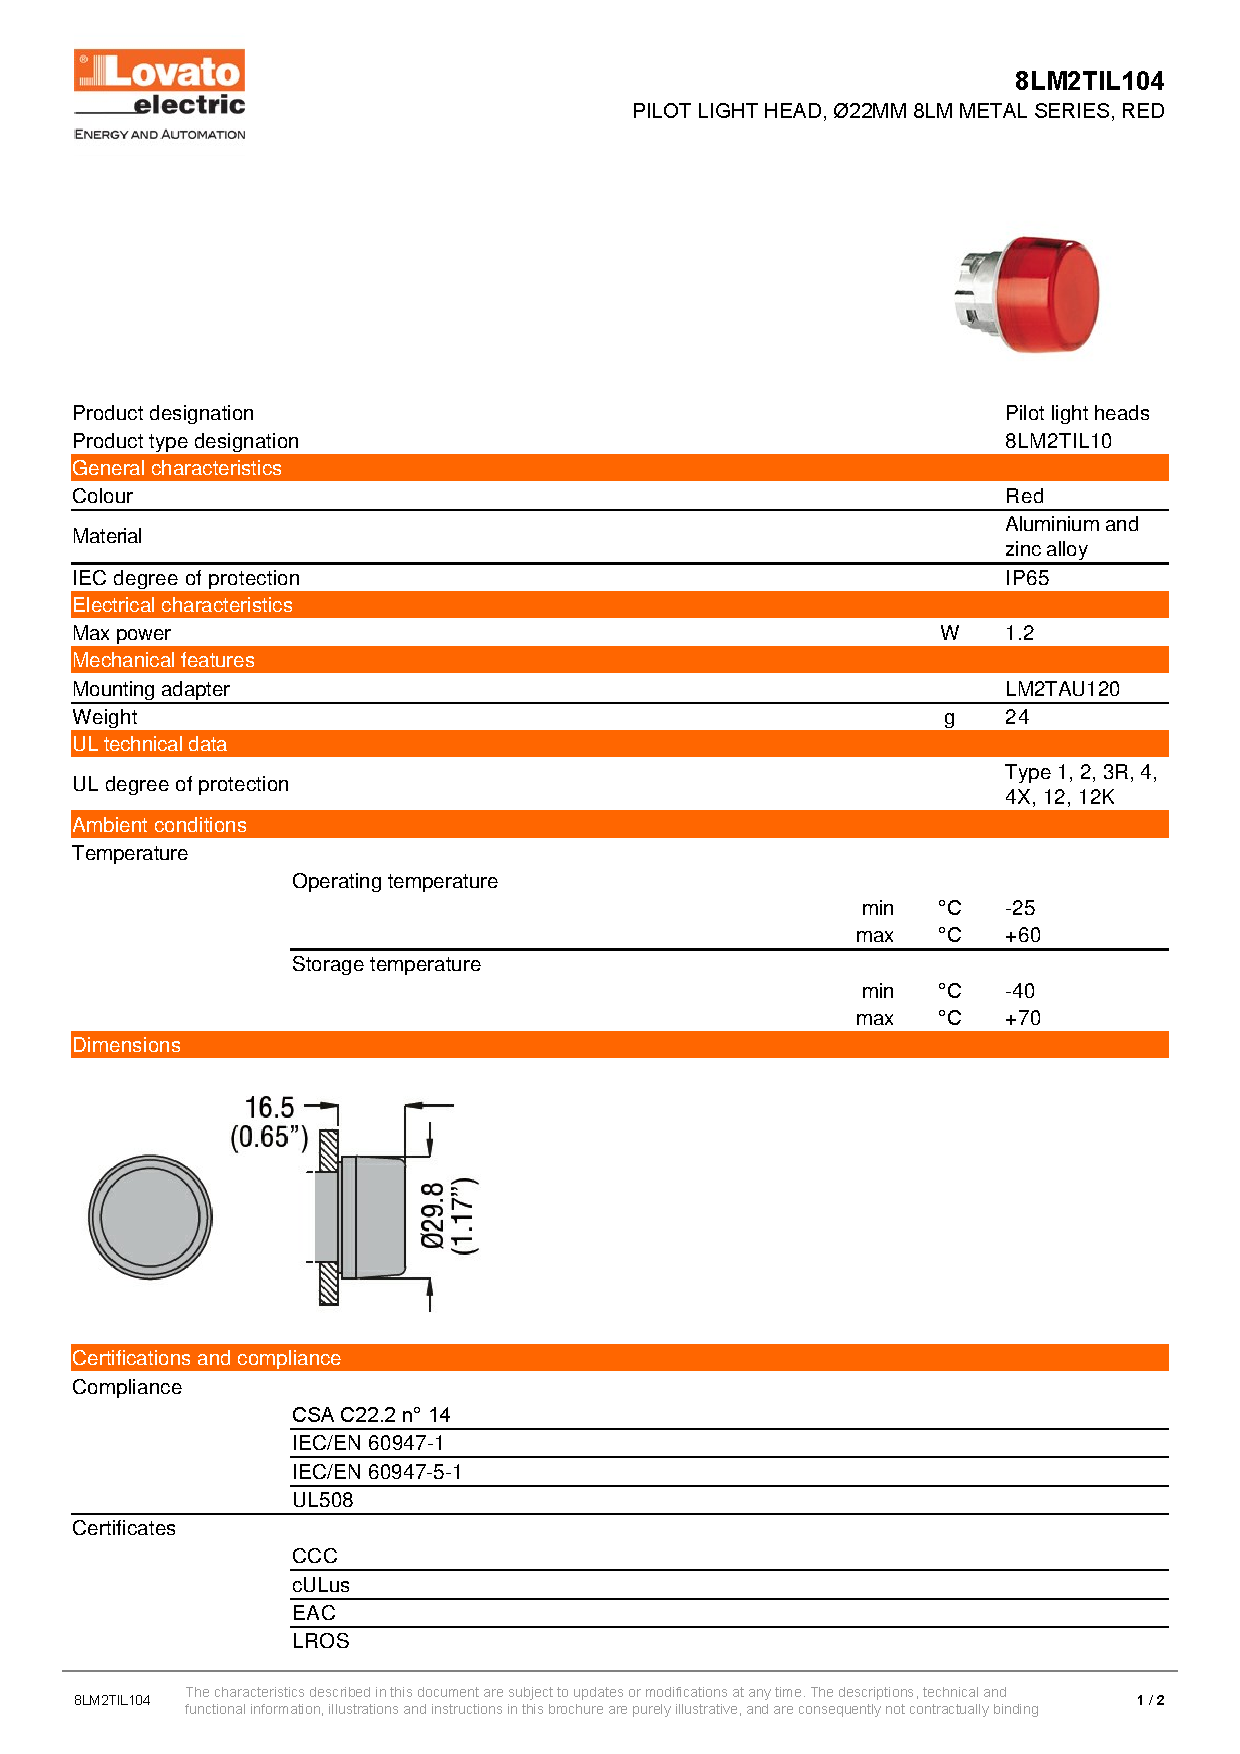
\includepdf[pages={-}, scale =1]{appendice/files/pilot_light_led_red.pdf}

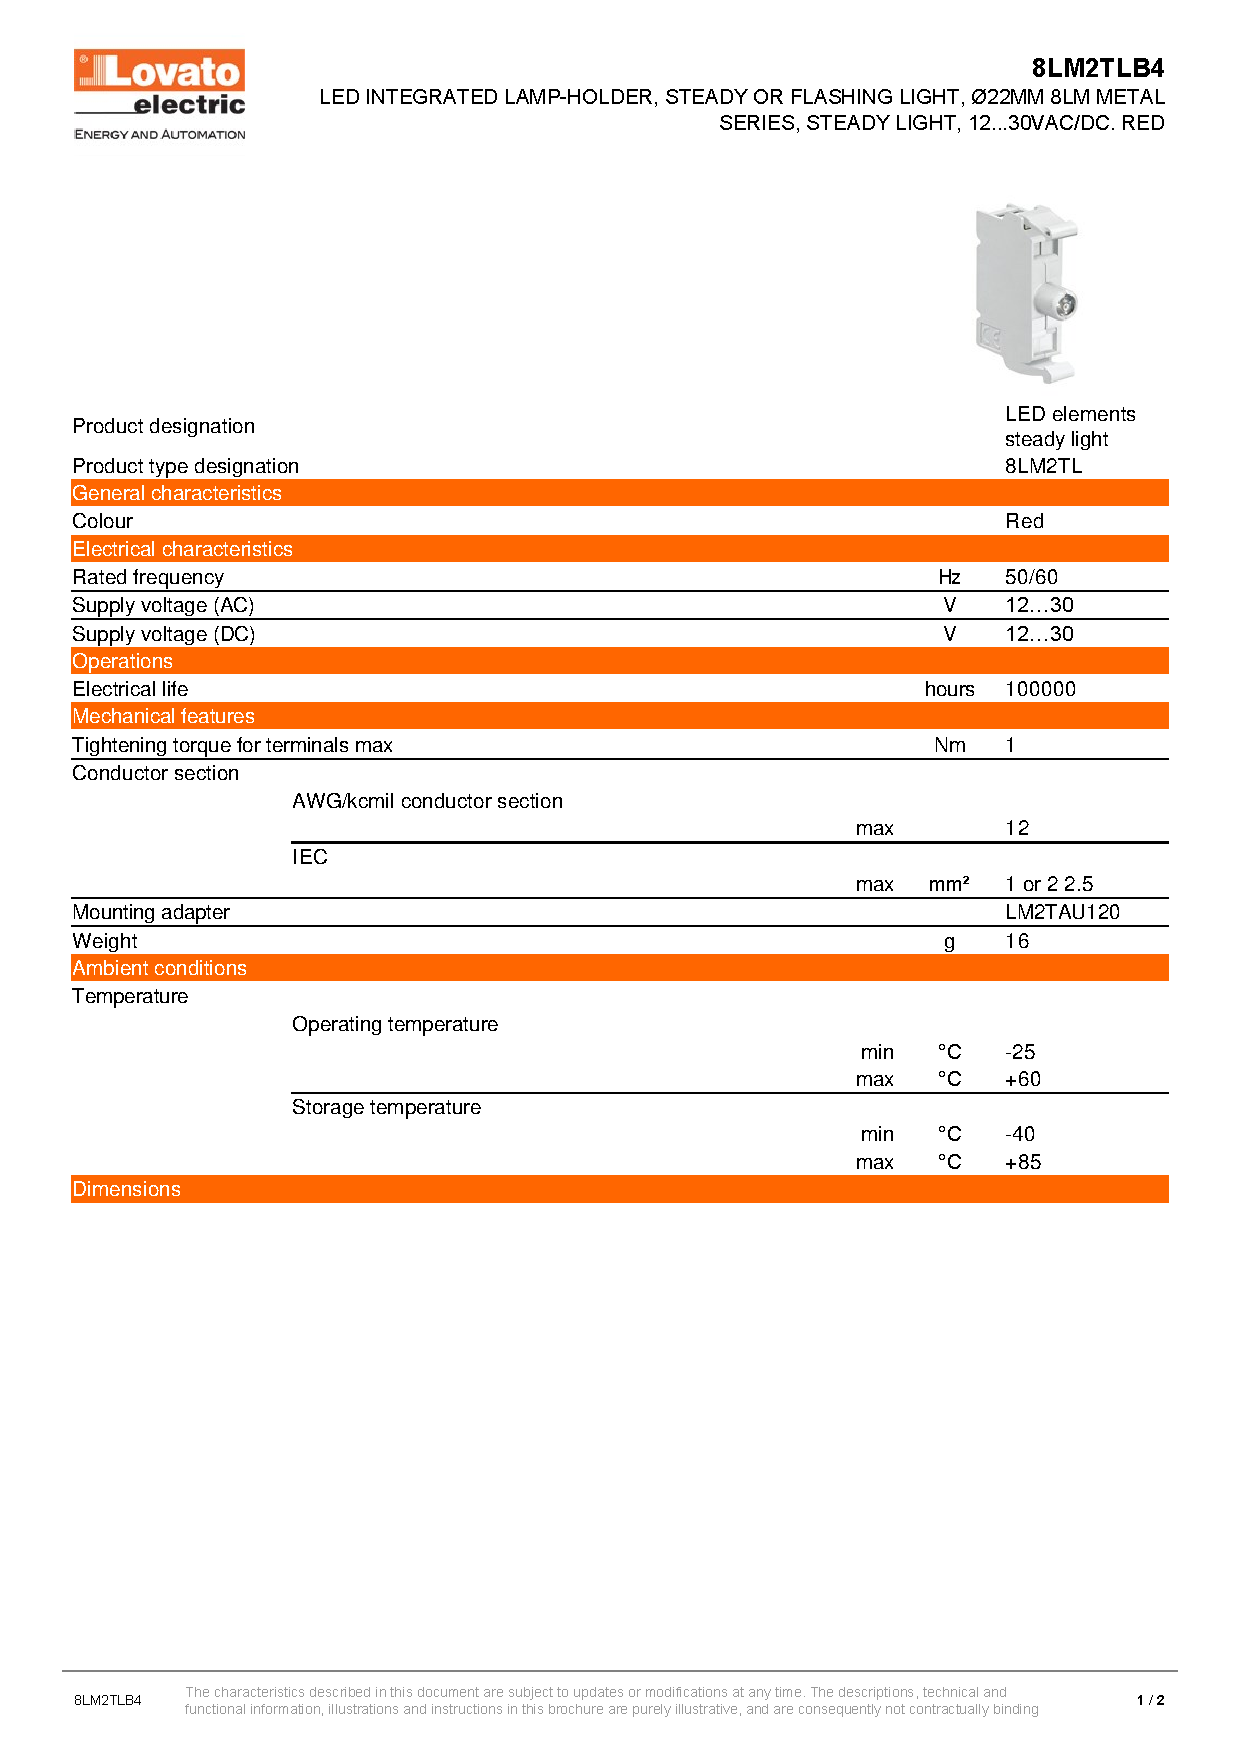
\includepdf[pages={-}, scale =1]{appendice/files/led_integrated_lamp_holder_red.pdf}

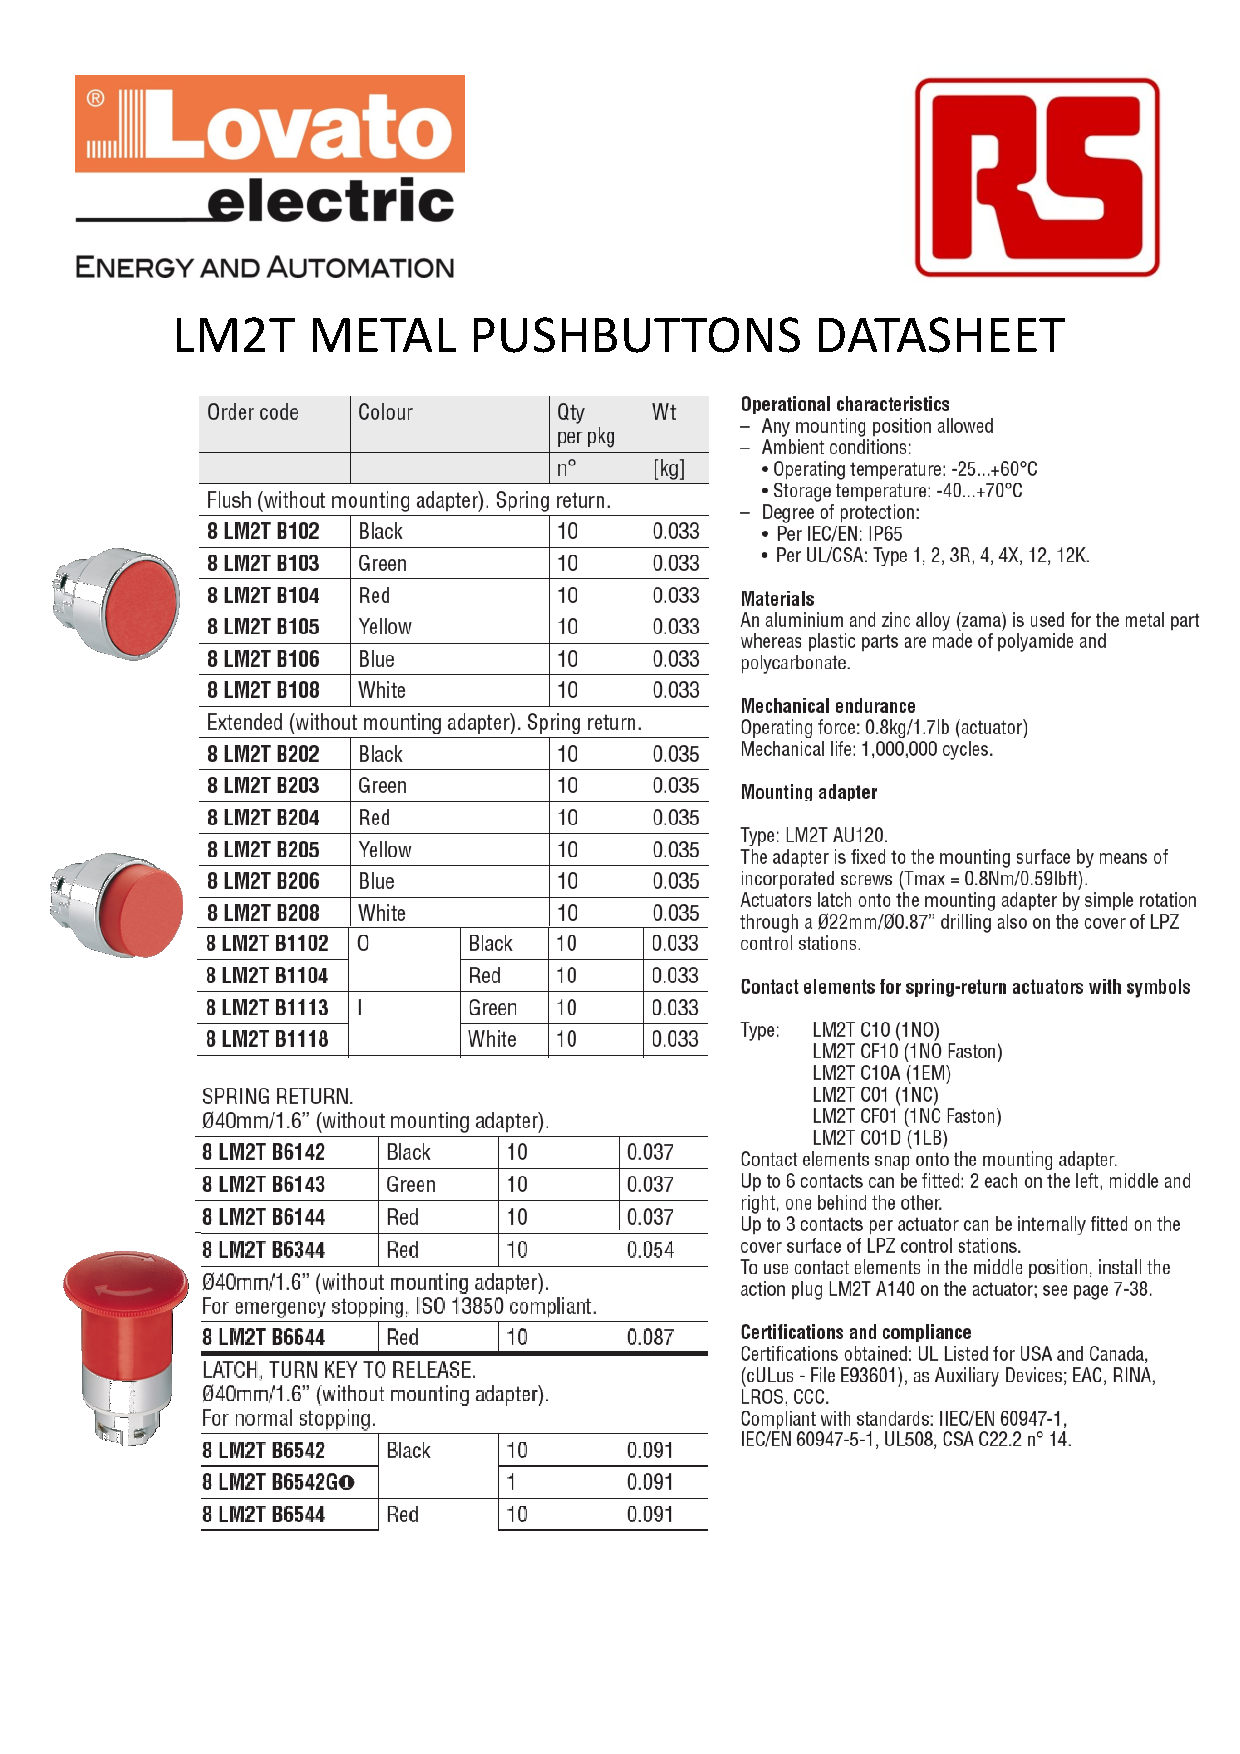
\includepdf[pages={1,3}, scale =1]{appendice/files/pushbutton.pdf}

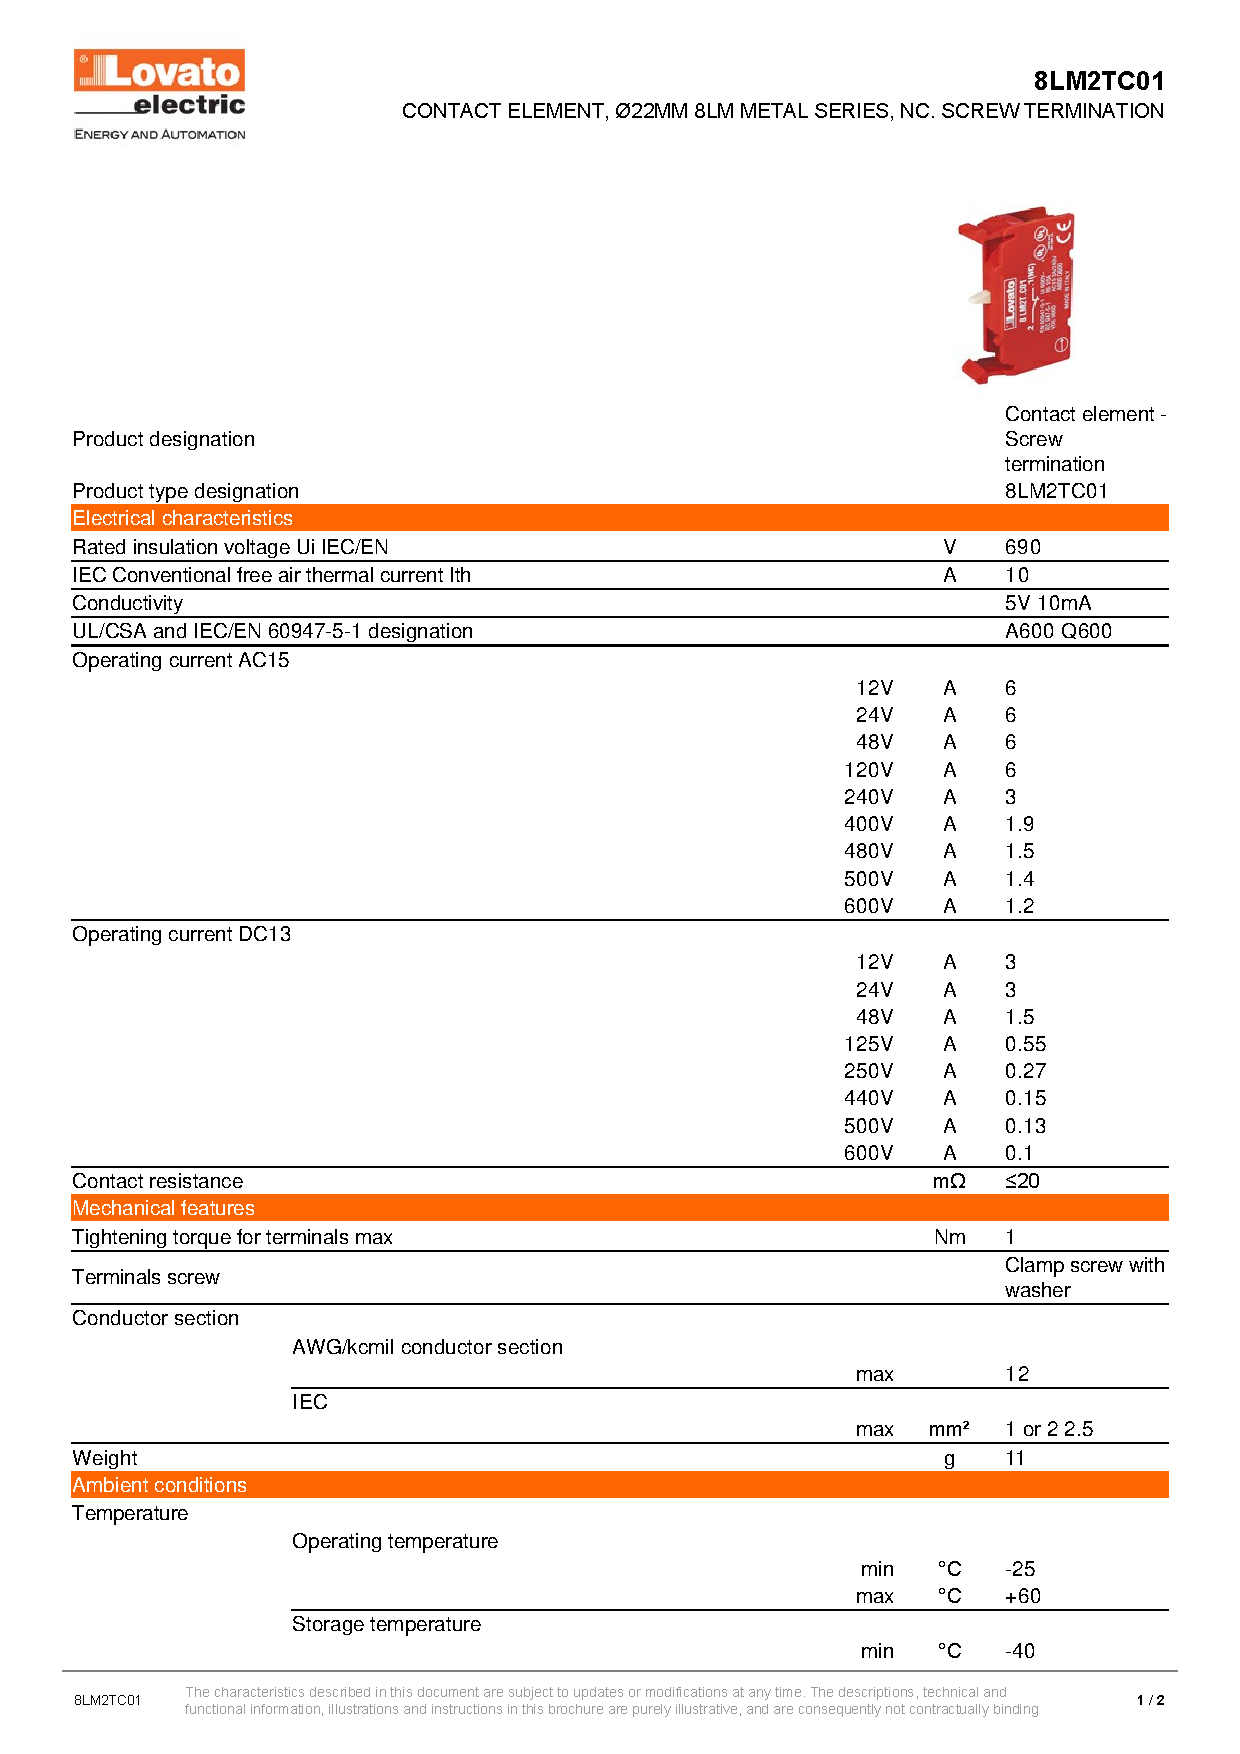
\includepdf[pages={-}, scale =1]{appendice/files/contact_element_nc.pdf}

\end{appendix}